
\documentclass[10pt]{ietbook}
\usepackage{listings}
%\usepackage{breqn}
\begin{document}

%For RH Book title
\rhbooktitle{Advances in Weather Radar}
%\setminted[python]{breaklines, framesep=2mm, fontsize=\footnotesize, numbersep=5pt}

\markboth{}

\cauthor{Mircea Grecu\thanks{GESTAR-II, Morgan State University and NASA GSFC} and\\
William S. Olson\thanks{GESTAR-II,UMBC and NASA GSFC} }

\chapter{Satellite Combined Radar-Radiometer algorithms}

Some abstract here.
\section{Introduction}

The benefit of incorporating radiometer observations into methodologies that estimate precipitation from
space-borne radar observations was first realized by \cite{weinman90}. Specifically, due to size and weight limitations on antennae, space-borne radars 
operate at frequencies that make observations subject to attenuation. While
attenuation correction methodologies exist, e.g. \cite{hitschfeld1954}, variability in the size distribution of
precipitation particles within the radar observing volume makes the attenuation correction process highly uncertain.
At the same time, it had been recognized \cite{Meneghini1983} that independent information regarding the Path-Integrated-Attenuation (PIA) 
may be used to reduce uncertainties in the attenuation correction process. PIA information
independent of the radar measurements used in the attenuation correction process may be derived from the analysis
of the electromagnetic power backscattered by the Earth's surface \cite{Meneghini1983} and, as noted by Weinman et al. \cite{weinman90}, 
low-frequency radiometer observations when available.  The objective of the surface analysis is to estimate the power backscattered by Earth's surface in the 
absence of the rain.  In the presence of rain, the ratio between the actual backscattered power and the estimated clear-sky backscattered power provides an estimate
of the total attenuation from the radar to the Earth's surface \cite{Meneghini1983} that can be used in attenuation correction and precipitation estimation process. 
The problem with the PIA estimation using this approach, usually referred to as the Surface Reference Technique (SRT), is that the estimation of the no-precipitation 
backscattered power may be highly uncertain in some situations.  As recognized by Weinman et al. \cite{weinman90} and even earlier investigators, e.g. \cite{Fujita1985},
radiometer observations over water surfaces at frequencies not associated with significant scattering (e.g. 10- and 19-GHz) contain information strongly related to the PIA.  
This is because the emissivity of water surface is low and rain drops in the radiometer observing volume result in warmer brightness temperatures.  The departure from the
brightness temperature value expected in clear skies may be used to estimate the equivalent PIA at the radar operating frequency \cite{weinman90}.  The initial study of
Weinman et al. \cite{weinman90} provided a relationship between coincident radiometer observations at X-band and the associated PIA at X-band (9.6-GHz). Subsequent work 
Smith et al. \cite{smith1997} was carried out to determine a relationship between the PIA at Ku-band (13.8 GHz) and coincident radiometer observations 10.7-GHz. 
This relationship was developed for use in the Tropical Rainfall Measuring Mission (TRMM) \cite{kummerow1998} combined radar-radiometer algorithm \cite{haddad1997}.

However, although the relationships between low frequency brightness temperatures and the radar PIA at X- and Ku-band are well-defined and unambiguous, the use of satellite
radiometer observations in satellite radar profiling algorithms is challenging. This because the typical footprints of low-frequency radiometer observations are significantly
larger than the typical footprints of space-borne radars, which makes the radiometer observations difficult to translate into radar PIA. To overcome this difficulty various
approaches akin to the downscaling of the radiometer observations to the radar footprint resolution have been developed \cite{haddad1997,grecu2004,masunaga2005,munchak2011}.
A common feature of these approaches was that the radar-footprint PIA was not directly estimated from the radiometer observations. Instead, 
optimization procedures were used to maximize the agreement between radiometer observations predicted from the radar observations and actual radiometer observations.  While
the impact of the radiometer observations on the final radar estimates is difficult to quantify, a clear benefit of combined radar-radiometer precipitation retrievals
are consistent with both the radar and radiometer observations.  Consequently, they may be used to derive large databases of precipitation and associated radiometer observations
necessary in the development of “Bayesian” precipitation estimation algorithms from satellite
radiometer-only observations \cite{grecu2006,kummerow2011,hou2014}. 

\section{Fundamental Models}

\subsection{Precipitation particles and their electromagnetic properties}

To numerically characterize integral properties of precipitation (such as the precipitation rate) within a radar observing volume, a good understanding of the 
distributions of properties such as the size and mass of precipitation particles is necessary.
Paramount to this is the concept of Particle Size Distribution (PSD).  Mathematically, the PSD is a function $N(D)$ that describes the density of precipitation particles of
a given size within an elementary atmospheric volume.  More precisely, $N(D)dD$ is defined as the concentration of precipitation particles with sizes between $D$ and $D+dD$
in a specified volume of air.  Given expressions that relate the size of a precipitation particle to its mass and electromagnetic backscattering
properties, the PSD function may be used to derive relationships between the Liquid Water Content (LWC) and radar reflectivity.  In a seminal
study, Marshall and Palmer  \cite{marshall_palmer_1948} showed that rain Drop Size Distributions (DSDs) follow an exponential distribution,
i.e. $N(D)=N_0\exp(-\lambda D)$.  Although subsequent studies showed that DSDs are generally better described by gamma functions,
$N(D)=N_0 D^{\mu}\exp(-\lambda D)$, (see Ulbrich 
\cite{ulbrich1983} for a review), the exponential DSD formulation of \cite{marshall_palmer_1948} represented a milestone in meteorology because
it set the stage for analytical investigations of the relationships between precipitation properties and radar observations.  While initially
focused preponderantly on rain, as measurement techniques improved, PSD studies started addressing ice particles in the early seventies 
(e.g. \cite{ssrivastava1970,heymsfield_a1977}). It was found that, similarly to raindrops, ice PSDs may be accurately described by gamma functions.

Equally important to the description of PSDs is the quantification of the amount of radar power backscattered by precipitation particles. 
To simplify the analysis, the radar measurements of returned power are converted into a related variable called the equivalent 
radar reflectivity factor, defined as \cite{meneghini1990}:

\begin{equation} \label{eq:Z}
Z=\frac {\lambda ^4} {\pi ^5 |K_w|^2} \int_0^{\infty} N(D) \sigma _b(D) dD
\end{equation}
where $\lambda$ is radar frequency, $|K_w|$ is the dielectric factor of water, and $\sigma _b(D)$ is the 
backscattering cross-section of a precipitation particle of diameter $D$.  The backscattering cross-section is the equivalent area that
would isotropically return an amount of power equal to that actually returned by the precipitation particle \cite{battan1973}.  
The equivalent reflectivity factor is defined to equal $\int_0^{\infty} N(D) D^6 dD$ (in mm${^6}$m$^{-3}$) for spherical rain drops
in the Rayleigh regime.  That is, for spherical raindrop whose diameter $D$ satisfy the inequality $\frac {\pi D} {\lambda} < 1$, the
backscattering cross-section $\sigma_b(D)$ is proportional to $D^6$.  For DSD characterized by raindrops in the Rayleigh regime, 
the radar reflectivity $Z$ defined $\int _0 ^{\infty} N(D) D^6 dD$ is a very simple but meaningful variable that can be calculated analytically
as a function of the DSD parameters and readily determined from the power measured by radar. Consequently, the radar reflectivity has
been established as the most meaningful and convenient variable to interpret the radar return power.  When the precipitation particles
do not fall in the Rayleigh regime, the general formulation given in Eq. (\ref{eq:Z}) is used to interpret observations.  It should be noted
that the conversion from
power to reflectivity (or equivalent reflectivity) is computationally the same, irrespective of whether precipitation particles are
in the Rayleigh regime or not.  However, the interpretation of observed radar reflectivity needs to account for the possibility of
the precipitation particles not being in the Rayleigh regime.

When raindrops are too large relative to the radar wavelength, the Mie solution of Maxwell's electromagnetic equations is generally used
to calculate $\sigma _b(D)$ \cite{bhmie2008}.  While the Mie solution assumes spherical scatterers, large raindrops are oblate.  
Although the assumption of spherical raindrops is acceptable in many situations, there are radar applications when the oblateness of 
raindrops needs to be considered.  In such applications, the electromagnetic properties of raindrops can be calculated using a 
more complex numerical methodology called the T-Matrix approach \cite{misch2002}. The use of the Mie solution in weather applications
dates back to at least 1961 \cite{battan1973}.

The quantification of the backscattering cross-section of ice particles is significantly more challenging than that of raindrops.
This is because ice-particles exhibit a large variety of complicated shapes that preclude the application of straightforward 
electromagnetic equation solvers such those used in the Mie and T-matrix approaches.
Before the emergence of computationally more general solvers, it was customary to assume that ice particles are spherical mixtures
of ice and air characterized by an equivalent dielectric constant \cite{battan1973}.  However, this assumption does not work well for
ice particles large compared to the radar wavelength \cite{tyynela2011,liu2004,kuo2016}. To address the need for accurate backscattering
calculations (and electromagnetic scattering properties in general), several research groups started developing databases of ice particles
and associated scattering properties using the Discrete Dipole Approximation (DDA) approach \cite{dda1994} 
and made them available to the science community at large \cite{liu2004,kuo2016}.  The drawback of DDA approach is its computational
cost. Specifically, the complexity of ice particle shapes precludes the use of efficient spectral solvers that make use of analytical formulae
that reduce the original equations to significantly simpler equations solvable in the Fourier space \cite{spectral_matlab}.  As a consequence, 
intensive numerical
calculations are necessary to quantify the electromagnetic properties of ice particles.  To circumvent the intensive numerical calculates, 
Hogan et al. \cite{hogan2017} developed an approach based on the Rayleigh-Gans approximation that provides computational efficient yet
accurate estimates of the electromagnetic properties of ice particles at microwave frequency.  When available, 
scattering calculations based on the DDA or other numerically intensive methods are preferable, but such calculations are not available at 
all frequencies, especially for new sub-millimeter wavelength radiometers that have been only recently developed or are being developed for
future space missions.  For such frequencies and very large ice particles relative to the instrument's wavelength,  the Rayleigh-Gans 
approximation of Hogan et al. \cite{hogan2017}  that together with the Mie-based approach of \cite{bhmie2008} and absorption models (e.g.
Rosenkranz \cite{rosenkranz1998}) provide the ingredients necessary to simulate space-borne radar and radiometer observations from 
atmospheric geophysical variables.

Although valuable insight can be derived from analytical formulations of the PSDs, the increased availability of PSD observations from field
campaigns eventually resulted in a paradigm shift regarding the use of the PSD observations in precipitation estimation methodologies.  Specifically,
it was found that a concentration scaling parameter $N_w$ can be derived from observations without any assumption regarding the PSD shape 
and used along with a geometric scaling parameter, i.e.
the volume weighted $D_m$, to accurately characterize all relevant PSDs and the associated radar and radiometer properties \cite{norm_dsd_2001}.  
The concentration scaling
parameter, also known as the generalized PSD intercept \cite{bringi2003}, is defined as
\begin{equation} \label{eq:nw}
    N_w=\frac {4^4} {\pi \rho_w} \frac {PWC} {D_m^4}
\end{equation}
where $PWC$ is the equivalent precipitation (either ice or rain) water content and $D_m$ is the volume (or mass) weighted diameter.  One of
the most consequential implications of the normalized intercept is the fact that it can explain and mitigate variability in the relationships between
radar observations and associated precipitation variables such as equivalent water content and rate.  
That is, representations of the joint distributions of reflectivities simulated from 
observed PSDs and the associated precipitation water content exhibit significant variability that makes the estimates the precipitation water content
from single frequency reflectivity observations highly uncertain.  Shown in the left-hand panel of Fig. \ref{fig:normZ} is the joint distribution of 
IWC and associated reflectivity at Ku-band calculated using PSD observations from the NASA IMPACTS field experiment \cite{impacts2022}.  As apparent 
in the panel, the joint distribution is broad with a broad range of IWC values associated with any given reflectivity.  However, normalization of 
both IWC and reflectivity by the associated $N_w$ makes the resulting joint ($IWC/N_w$, $Z(Ku)/N_w$) very narrow and close to a one-to-one function.
This means that $IWC/N_w$ can be accurately predicted from $Z(Ku)/N_w$.  While normalization by itself does not eliminate uncertainties, because one
needs information about $N_w$ to derive a closed form solution for $IWC$, it does provide a general and physical consistent 
framework to investigate and mitigate uncertainties in space-borne radar and radiometer retrievals.  This will be explained in detail in the next 
section.  A remarkable fact regarding the normalization by $N_w$ is that it collapses all radar-precipitation relationships (e.g. reflectivity vs precipitation
rate, attenuation vs reflectivity, attenuation vs. precipitation rate etc.) to one-to-one functions for both ice and water \cite{ferreira2001}.


\begin{figure} 
\centerline{ }
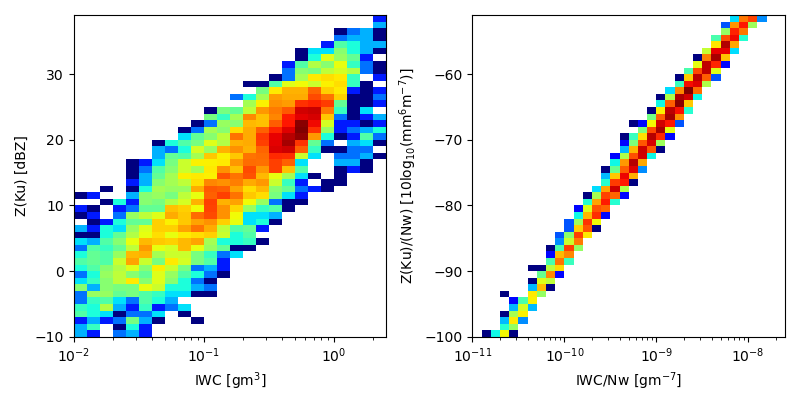
\includegraphics[width=\textwidth]{normZvsnormIWC.png}

\caption{ (Left) joint distribution of ice water content (IWC) and associated Ku-band reflectivity calculated from PSD observations from IMPACTS and
(Right) joint distribution of normalized IWC and Ku-band reflectivity. }
\label{fig:normZ}
\end{figure}

\subsection{Radar and radiometer models}
The measured radar reflectivity at range $r$ can be expressed as a function of the true radar reflectivity at range $r$, $Z(r)$, and the integrated attenuation
along the path \cite{iguchi_meneghini_1994}.
\begin{equation}\label{eq:radarEq}
Z_m(r)=Z(r) \exp(-0.2\ln(10)\int_0^r k(Z(s))ds)
\end{equation}
where $k(Z(s))$ is the specific attenuation at range $s$.  The specific attenuation may be determined as a function of an observed or assumed analytical PSD
using an equation similar to Eq. (\ref{eq:Z}), i.e. $k=\int_0^{\infty} N(D) \sigma_e(D)dD$, with the extinction cross-section $\sigma_e(D)$ determined using one of
the electromagnetic computational methodologies described in the previous section.  When the specific attenuation and the reflectivity are related through a 
power law, i.e. $k=\alpha Z^\beta$ with $\beta$ constant with range, a closed form solution for $Z$ exists \cite{iguchi_meneghini_1994}, i.e.
\begin{equation}\label{eq:hbsol}
Z(r)=Z_m(r) /(1-q\int_0^r Z_m^\beta(s)ds)^{1/\beta}
\end{equation}
where $q=0.2\beta ln(10)$.  This solution was first derived by Hitschfeld and Bordan \cite{hitschfeld1954} and started
getting prominent in spaceborne radar applications with the work of \cite{meneghini1983}, \cite{marzoug1991} 
and \cite{iguchi_meneghini_1994}.

A particular challenge in applying Eq. (\ref{eq:hbsol}) to radar observations affected by significant attenuation is
that the numerical value of term $q\int_0^r Z_m^\beta(s)ds$ may become larger than 1.0, in which case the equation
is not applicable anymore. Moreover, even if $q\int_0^r Z_m^\beta(s)ds<1$ the path integrated attenuation associated
with Eq. (\ref{eq:hbsol}) may not be in agreement with estimates from a Surface Reference Technique (SRT) analysis.  This
is discussed in \cite{marzoug1991} and \cite{iguchi_meneghini_1994}.  Several ad-hoc techniques were developed to 
reconcile solution \ref{eq:hbsol} with the SRT estimates, but, fundamentally, the problem was not satisfactorily 
addressed from the physical perspective until the work of Ferreira et al. \cite{ferreira2001}. 
Ferreira et al. \cite{ferreira2001} noted that all $k-Z$, $Z-R$ or $Z-PWC$ (where $k$ is the specific attenuation
and $Z$, $R$ and $PWC$ are the associated reflectivity, precipitation rate and precipitation water content) are 
exact for a given constant $N_w$.  They also noted that more general relationships, explicitly accounting for the $N_w$
variability, need to be derived and used to make the Hitschfeld-Bordan 
solution in Eq. (\ref{eq:hbsol}) consistent with SRT estimates of Path Integrated Attenuation (PIA).  Specifically,
a more general $k-Z$ relationship of the type
\begin{equation} \label{eq:kZ}
k=dN_w^{1-\beta} \alpha Z^{\beta}
\end{equation}
where $dN_w$ is the ratio of actual $N_w$ to that of the reference $N_{w}^0$ for which the relation $k=\alpha Z^{\beta}$ 
holds perfectly may be derived and used with \ref{eq:hbsol}.  The PIA attenuation associated with the generalized 
$k-Z$ relation in  \ref{eq:kZ} is
\begin{equation} \label{eq:PIA}
PIA_{HB}(dN_w)=-10/\beta \log_{10}(1-q dN_w^{1-\beta} \int_0^{r_s}\alpha Z_m^\beta(s)ds)
\end{equation}
Given an independent estimate of PIA from the SRT, $PIA_{SRT}$, one may determine the value of $dN_w$ that satisfy
$PIA_{HB}(dN_w)=PIA_{SRT}$.  This provides a physical approach to reconcile the Hitschfeld-Bordan solution with a potentially
different SRT PIA estimate \cite{ferreira2001}.  The benefit of this approach relative to more ad-hoc approaches such
as the $\alpha$ adjustment method \cite{iguchi_meneghini_1994} is that it enables the adjustment of the $Z-R$ 
(or $Z-PWC$) used in the estimation of precipitation rates (or equivalent water contents) from the attenuation corrected
reflectivities \cite{ferreira2001}. This is because systematically different mean particle sizes may result not only
in biased attenuation correction,  but also in biased precipitation estimates due to the application of a biased reflectivity
precipitation relationship.  Therefore, the benefit of using $N_w$-based relationships is twofold \cite{ferreira2001}.

It should be noted that because neither the SRT estimates nor the Hitschfeld-Bordan predictions of PIA are perfect,
equating them exactly is suboptimal because it attributes various types of uncertainties to variability in the $N_w$.
A better approach is to adjust $N_w$ such that the final $PIA_{HB}$ is consistent with both the uncertainties in its
initial values (prior to the SRT based adjustment) and the $PIA_{SRT}$ uncertainties. Iguchi et al. \cite{iguchi2000}
developed such a methodology based on Bayes estimation theory. However, Iguchi et al. \cite{iguchi2000} did not update
the Hitschfeld-Bordan solution in terms of $N_w$, but in terms of an equivalent variable $\epsilon$, and it was Ferreira
et al. \cite{ferreira2001} who made the connection between SRT estimates and $N_w$ adjustments.

The use of normalized $k-Z$ and $Z$-precipitation relation is beneficial even when SRT PIA estimates are not available
but additional sources of information, such as coincident radiometer observations are available.  Specifically, if a
set of observations $Y_obs$ independent of the radar observations used in a radar-only precipitation profiling algorithm,
one may tune the $N_w$ assumptions made in the radar-only profiling algorithm to maximize the agreement between
them and their prediction from the radar-only estimates.  Or, more precisely, an objective function may be defined as 
\begin{multline} \label{eq:fobj}
    F(\mathbf{N_w})=\frac {1}{2} \mathbf{(Y_{obs}-Y(Z_m(N_w)))^T W_Y^{-1} (Y_{obs}-Y(Z_m(N_w)))} +\\
    \frac {1} {2} \mathbf{(N_w-N_w^0)^T W_N^{-1} (N_w-N_w^0)}
\end{multline}
where $\mathbf{Y(Z_m(N_w))}$ is a numerical model that predicts observations $\mathbf{Y_{obs}}$ as a function of the space-borne
radar observations $\mathbf{Z_m}$ and the normalized $\mathbf{N_w}$ intercepts. Matrix $\mathbf{W_Y^{-1}}$ quantifies uncertainties
in model $\mathbf{Y}$, while $\mathbf{N_w^0}$ and $\mathbf{W_N}$ are the climatological values of $\mathbf{N_w}$ and their 
associated covariance matrix.
Note that $\mathbf{Y_{obs}}$ may consist of any useful combination of space- or ground-based observations, while the set of $N_w$ may
need to be extended to include other geophysical variables relevant in the prediction of $\mathbf{Y}$.  From the mathematical perspective,
the problem of determining $\mathbf{N_w}$ from $\mathbf{Y_{obs}}$ is generally ill-posed and additional climatological, or 
"a priori" in statistical terminology, information is needed to derive a unique solution \cite{tarantola2005}.  The additional information
is provided by the second term of the objective function in Eq. (\ref{eq:fobj}). An implementation of a combined radar-radiometer estimation
algorithm based on Eq. (\ref{eq:fobj}) and applicable to airborne observations was developed by Grecu and Anagnostou \cite{grecu2002}.
An evaluation based on synthetic observations derived from cloud resolving model simulations indicated the superiority of the relative
to radar-only retrievals.  A potentially more general approach, i.e. considering a larger set of state variables, but computationally 
more intensive and prone to challenges when used in operational environment had been developed by Marzano et al. \cite{marzano1999}.
Specifically, the state variables in \cite{marzano1999} included the precipitation water contents while the radar observations were 
not implicitly satisfied but included in the optimization problem.  A comprehensive discussion on why an approach with a reduced number
of variables and the radar observations at a given frequency automatically satisfied in provided in \cite{grecu2002}.

Irrespective of whether single-frequency radar observations are included in the objective function or automatically satisfied, it should
be noted that the use of additional information enables in theory the derivation of more accurate estimates of additional variables, such
as the normalized PSD intercepts, that in the worst case scenarios are simply set up based on their climatology. To estimate the state
variables in Eq. (\ref{eq:fobj}), a computationally efficient model to simulation the observations $\mathbf{Y}$ and an optimization procedure
are needed.  The simulation of air- and space-borne radiometer requires a procedure to solve the radiative transfer equation, which
in the plane-parallel approximation reads \cite{kummerow1993}.
\begin{multline}\label{eq:rte}
\mu k_{ext}\frac {dI(\mu,\phi)}{dz}=-I(\mu,\phi) + (1-a)B(T)+\\
\frac {a} {4\pi} \int_0^{2\pi}\int_{-1}^{1}p(\mu,\phi,\mu',\phi')I(\mu',\phi')d\mu'd\phi'
\end{multline}
where $I(\mu,\phi)$ is the intensity in direction given by $\mu$ (the cosine of the angle between the actual direction and 
the vertical axis) and azimuthal angle $\phi$, $k_{ext}$ is the extinction coefficient, $a$ is the scattering albedo (the ratio
of the scattering coefficion to the extinction coefficients), $B(T)$ is the black body radiation emitted by the atmosphere at 
temperature $T$ and the radiometer's frequency and $p(\mu,\phi,\mu',\phi')$ is the scattering function. The most general solvers
of the radiative transfer equation are computationally intensive.  However, the assumption of no azimuthal dependence and the
approximation of $I$ and $p(\mu,\mu')$ using the first two terms of a Legendre series \cite{kummerow1993} reduce the initial equation
to a system of two coupled ordinary differential equations \cite{kummerow1993}.  Systematic evaluations between the approximate solution
and more general solutions revealed differences that can mitigate through simple modifications that account for geometric effects in
the approximate solution \cite{liu1996}.

The relevant coefficients in Eq. (\ref{eq:rte}) are determined through the integration of the absorption, scattering and phase function
properties of individual particles for given observed or analytical PSDs. A file containing the integrated scattering properties used in 
the Global Precipitation Measurement (GPM) combined algorithm \cite{grecu2016} is available in netCDF format at:\\
https://github.com/mgrecu35/IET\_bookChapter/tree/main/lookupTables.
The properties of four types of hydrometeors, i.e. rain, snow, graupel and hail, are included in the file. Properties are calculated assuming
normalized gamma particle size distributions with $\mu$=2 and $N_w$=0.08cm$^{-4}$.  The mean mass diameter, precipitation rate,
and precipitation water content associated with each entry are also included in the file. The rain, graupel and hail properties are calculated using
the Mie approach, while the snow properties are derived from DDA calculations. Additional information is provided in the README.md in the lookup table
directory. An implementation of plane-parallel radiative solver of the \cite{kummerow1993} is available in directory src of 
https://github.com/mgrecu35/IET\_bookChapter/.  The reader is encouraged to pull the entire directory and examine the files in subdirectory examples.
These files provide examples of radar and radiometer calculations using the concepts described in the chapter.  The examples require an working
version of Python and some specific library.  Instructions on how the installation of the required library are provided in the README file
in the examples directory.

\subsection{Elements of optimal estimation theory}

According to Gelb \cite{gelb1974}, an optimal estimator is a computational algorithm that processes measurements to deduce a minimum error (in accordance with some
stated criterion of optimality). Based on this classical definition, any estimate that results from the minimization of an error-related objective function like the
that in Eq. (\ref{eq:fobj}) is optimal. Nevertheless, because the minimization of observations errors is usually insufficient in deriving accurate estimates, additional
terms called regularization terms \cite{doicu2010} need to be included in the objective functions.  An effective and meaningful type of regularization may 
be achieved through the use of Bayes' Theorem \cite{maahn2020}.  Bayesian optimal estimation is preferable to other types of regularizations when the variables
to be estimated have well-defined physical models and their statistical properties may be systematically studied independently of the estimation problem at hand.
This is the case for combined radar radiometer retrievals because the distributions of PSD intercepts can be independently studied and characterized using
ground observations and/or numerical models.

Another element specific of optimal estimation procedure is their reliance on an optimization procedure. This is the reason why optimal estimation procedures
are not always the method of choice in applications.  Specifically, in some applications, the optimization problem  associated with the estimation problem is
so complicated that alternative (theoretically inferior) approaches are preferred.   

The ensemble smoothing algorithm may be summarized as follows:
\begin{itemize}
    \item Generate an ensemble of PSD intercepts $\mathbf{N_w}$.
    \item Derive radar-only precipitation estimation from the Ku-band radar observations.
    \item Simulate radiometer, additional frequency radar (if multiple radar observations are available) and SRT PIA observations.
    \item Apply an Ensemble Kalman Smoother
    \begin{equation}
        \mathbf{X=X+cov\langle X,Y \rangle (cov\langle Y,Y \rangle +R)^{-1} (Y_{obs}-Y(X))}
    \end{equation}
    to update the solution.
\end{itemize}

\subsection{Additional matters}
\subsubsection{Non-uniform beam filling}
\subsubsection{Multiple-scattering}
\subsubsection{Radiance preprocessing}
\section{Example of GPM combined observations and retrievals}
Shown in figure \ref{fig:dataEx} is an example of observations from the Global Precipitation Measurement (GPM) mission \cite{gail2017}.
Specifically, observed reflectivity from the Dual Frequency Precipitation Radar (DPR) and two of the associated brightness temperatures
from the GPM Microwave Imager (GMI) \cite{gail2017} for a portion of orbit 5866 over the Kwajelein atoll are shown. 
As apparent in the figure, at reflectivity observations tend to be significantly attenuated 
at Ka-band. Some scans exhibit attenuation even at Ku-band.  As discussed in the previous sections, the reflectivity observations need
to be corrected for attenuation to be usable in the derivation of precipitation estimates. Independent estimates of the PIA from the application
of SRT method are extremely important in the attenuation correction process.  However, reliable SRT PIA estimates are not always available,
especially when only single frequency radar-observations are available and the attenuation is low relative to the noise in the estimates.
An assessment of the accuracy of the DPR PIA estimates from the single and dual frequency SRT method is provided in \cite{meneghini2015}.
The 18.7-GHz brightness temperatures for orbit 5866 over the Kwajelein atoll are also shown in the bottom panel of Fig. \ref{fig:dataEx}.
As explained in the previous section brightness temperatures at X-band and higher frequencies may be used to estimate provide alternative PIA
estimates.  Such estimates are especially useful when the SRT PIA estimates are unreliable. However, they may be used in the estimation process along 
with SRT PIAs, because the optimal estimation theory can effectively incorporate information from multiple sources as long as their uncertainties are 
properly specified.  The 18.7-GHz brightness temperatures are in qualitative agreement with the radar observations, i.e. they tend to increase
in regions where the radar observations suggest high intensity precipitation and significant attenuation and attain their minimum values in regions
where the radar does not detect any precipitation.  However, the 18.7-GHz exhibit significantly smoother along track variability than the radar
observations.  This is because the GMI's footprint size at 18.7-GHz is significantly coarser than the DPR's footprint size. Specifically,
the GMI's footprint resolution is 15.0 at 18.7-GHz \cite{gmi2015}, while that of the DPR is 4.5km.  As described in the previous section,
various approaches such as deconvolution or the convolution of DPR footprint simulated brightness temperatures and the evaluation of brightness
temperatures errors at the radiometer's footprint resolution may be used to account for the radar and radiometer's footprint size discrepancies.

\begin{figure} \label{fig:dataEx}
    \centerline{ }
    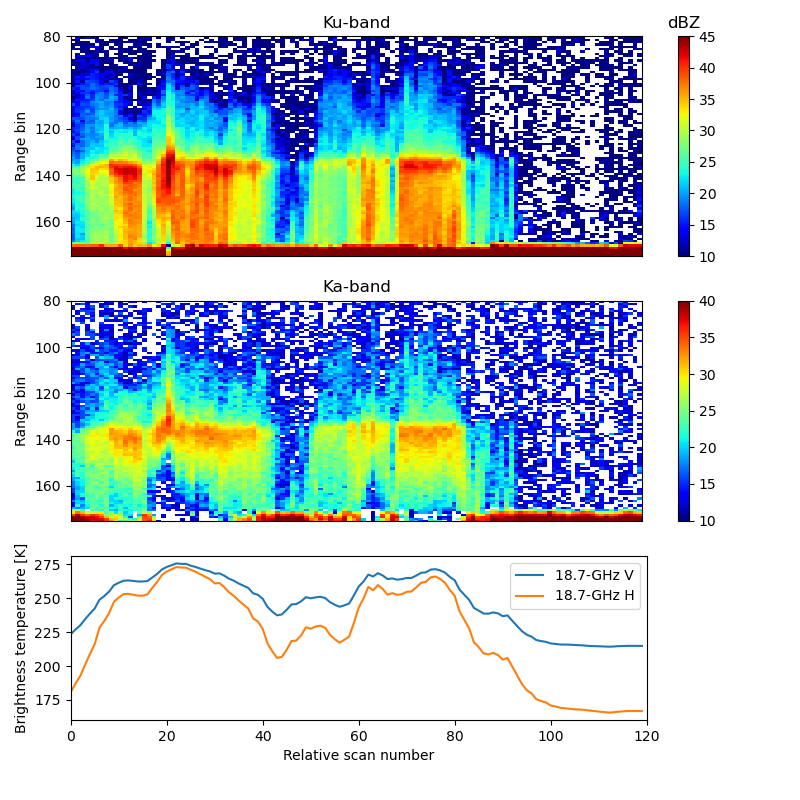
\includegraphics[width=\textwidth]{kwajObs.20150311-S162503-E162626.005866.png}
    
    \caption{Example of observed DPR Ku-(top), Ka-band reflectivities (middle), and GMI 18.7-GHz brightness temperatures (bottom).}
\end{figure}

\subsection{Machine learning based evaluation}
Insight into the utility of brightness temperature information into the estimation of the PIA may be derived using a Machine Learning (ML)
approach.
\begin{figure} \label{fig:ML_PIA}
    \centerline{}
    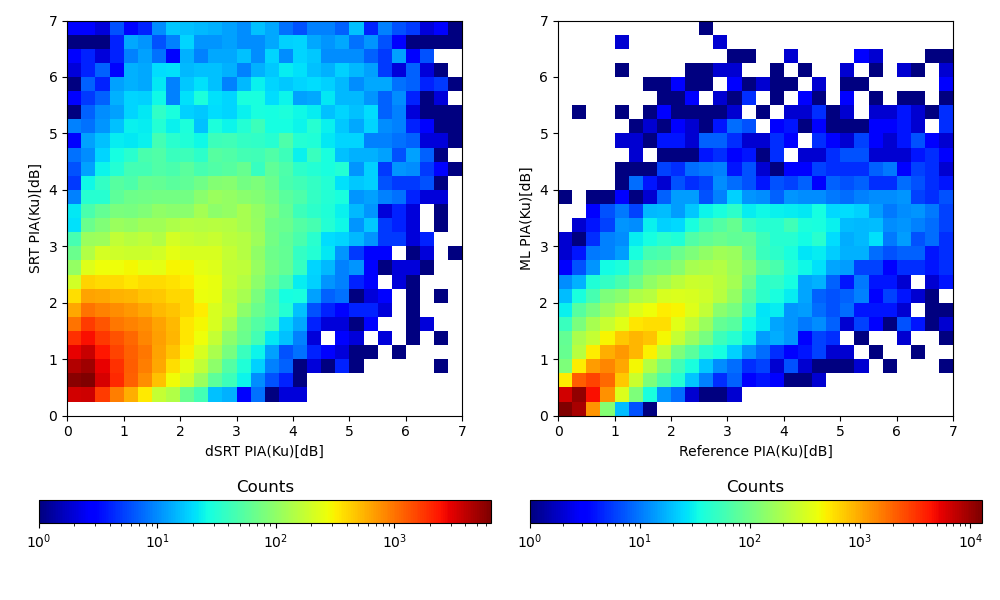
\includegraphics[width=\textwidth]{ML_PIA.png}
    
    \caption{(Left) Ku-band PIA estimates from the single frequency SRT analysis against Ku-band PIA estimates from the single frequency SRT analysis. Brightness-
    temperature ML-based PIA estimates against reference PIA estimates from both single and dual-frequency SRT analysis.}
\end{figure}

\section{Summary and conclusions}
%µdI(µ, φ)dτ= I(µ, φ) −˜ω4π2π01−1p(µ, φ; µ, φ)I(µ, φ) dµdφ

%F(N_w)=\frac {1}{2}  W_Y^{-1} ) 

% + \frac {1} {2} (N_w-N_w^0)^T W_N^{-1} (N_w-N_w^0)



%\begin{table}[!tb]
%\caption{A table}
%\processtable{ Example of code }
%\lstset{language=Python}
%\lstset{frame=lines}
%\lstset{caption={Insert code directly in your document}}
%\lstset{label={lst:code_direct}}
%\lstset{basicstyle=\footnotesize}
%\begin{lstlisting}
%from brg.datastructures import Mesh
 
%mesh = Mesh.from_obj('faces.obj')
%mesh.draw()
%\end{lstlisting}
%\end{table}

%\subsection{B heading (level 2)}

%\subsubsection{C heading (level 3)}

%\begin{figure}[!b]
%\centerline{\fbox{\hbox to 20pc{\vbox to 10pc{}}}}
%\caption{little figure here}
%\end{figure}

%\paragraph{D heading (level 4)}



\bibliographystyle{vancouver-modified}
\bibliography{sample-vancouver}

\end{document}
